
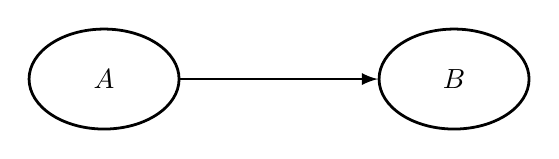
\begin{tikzpicture}[>=latex,line join=bevel,]
  \pgfsetlinewidth{1bp}
%%
\pgfsetcolor{black}
  % Edge: A -> B
  \draw [->] (54.03bp,18.0bp) .. controls (71.928bp,18.0bp) and (95.651bp,18.0bp)  .. (125.58bp,18.0bp);
  % Node: A
\begin{scope}
  \definecolor{strokecol}{rgb}{0.0,0.0,0.0};
  \pgfsetstrokecolor{strokecol}
  \draw (27.0bp,18.0bp) ellipse (27.0bp and 18.0bp);
  \draw (27.0bp,18.0bp) node {$A$};
\end{scope}
  % Node: B
\begin{scope}
  \definecolor{strokecol}{rgb}{0.0,0.0,0.0};
  \pgfsetstrokecolor{strokecol}
  \draw (153.0bp,18.0bp) ellipse (27.0bp and 18.0bp);
  \draw (153.0bp,18.0bp) node {$B$};
\end{scope}
%
\end{tikzpicture}

